\documentclass{beamer}
\mode<presentation>
\usepackage{amsmath}
\usepackage{amssymb}
\usepackage{mathtools}
\usepackage{listings}
\usepackage{graphicx}
\usepackage{hyperref}
\usetheme{Boadilla}
\usecolortheme{lily}

\setbeamertemplate{footline}{
  \leavevmode%
  \hbox{%
    \begin{beamercolorbox}[wd=.9\paperwidth,ht=2.25ex,dp=1ex,left]{author in head/foot}%
      \hspace{1em} Arnav Makarand Yadnopavit
    \end{beamercolorbox}%
    \begin{beamercolorbox}[wd=.1\paperwidth,ht=2.25ex,dp=1ex,right]{author in head/foot}%
      \insertframenumber{} / \inserttotalframenumber\hspace*{2ex}
    \end{beamercolorbox}}%
}
\setbeamertemplate{navigation symbols}{}

\numberwithin{equation}{section}
\title{10.4.1.2.3: Solving Rohan's Age Problem}
\author{EE24BTECH11007 - Arnav Makarand Yadnopavit}
\date{\today}

\begin{document}

\begin{frame}
\titlepage
\end{frame}

\section*{Outline}
\begin{frame}
\tableofcontents
\end{frame}

\section{Question}
\begin{frame}
\frametitle{Question}
Rohan's mother is 26 years older than him. The product of their ages (in years) 3 years from now will be 360. Find Rohan's present age.
\end{frame}

\section{Solution}
\subsection{Theoretical Solution}
\begin{frame}
\frametitle{Theoretical Solution}
Let Rohan's age, \( R = x \). Then Mother's age, \( M = x + 26 \). After 3 years, we have:
\[
(M + 3)(R + 3) = 360,
\]
\[
(x + 29)(x + 3) = 360,
\]
\[
x^2 + 32x - 273 = 0.
\]
Solving this quadratic equation:
\[
x = 7 \quad \text{or} \quad x = -39.
\]
Since age cannot be negative, Rohan's present age is:
\[
\boxed{7}.
\]
\end{frame}

\subsection{Computational Solution}
\begin{frame}
\frametitle{Computational Solution: Matrix-Based Method}
The quadratic equation is:
\[
x^2 + 32x - 273 = 0.
\]
Construct the companion matrix:
\[
A = \begin{bmatrix}
    0 & 1 \\
    -273 & -32
\end{bmatrix}.
\]
The eigenvalues of \( A \) are the roots of the polynomial.
\end{frame}

\subsection{QR Decomposition}
\begin{frame}{QR Decomposition}
QR decomposition factors a given matrix \( A \) into:
\[
A = QR,
\]
where \( Q \) is an orthogonal matrix \( Q^T Q = I \), and \( R \) is an upper triangular matrix.
\end{frame}

\subsection{Householder Transformations}
\begin{frame}{Householder Transformations}
Householder transformations are used to zero out elements below the diagonal of a matrix column. Given a vector \( v \), the Householder matrix is:
\[
H = I - 2 \dfrac{vv^T}{v^T v}.
\]

The process:
\begin{itemize}
    \item Initialize \( Q \) as the identity matrix.
    \item Let \( \vec{x} \) be the first column of \( A \), and \( \alpha = \|\vec{x}\| \).
    \item Compute:
    \[
    \vec{u} = \vec{x} - \alpha \vec{e}_1, \quad \vec{v} = \dfrac{\vec{u}}{\|\vec{u}\|}, \quad Q = I - 2 \vec{v}\vec{v}^T
    \]
    \item Result: \( Q_1 A \) transforms \( A \) to:
    \[
    Q_1 A = 
    \begin{bmatrix}
    \alpha_1 & * & \dots & * \\
    0 & & & \\
    \vdots & & A' & \\
    0 & & &
    \end{bmatrix}
    \]
\end{itemize}
\end{frame}

\begin{frame}{Householder Transformations}
This process is repeated for \( A' \) (obtained from \( Q_1 A \) by deleting the first row and column), resulting in \( Q'_2 \). Expand \( Q'_2 \) to \( Q_k \):
\[
Q_k = \begin{bmatrix} I_{k-1} & 0 \\ 0 & Q'_k \end{bmatrix}
\]

After \( n-1 \) iterations:
\[
R = Q_{n-1} \dots Q_2Q_1A, \quad Q^T = Q_{n-1} \dots Q_2Q_1, \quad Q = Q_1Q_2 \dots Q_{n-1}.
\]
\end{frame}

\subsection{QR Algorithm for Eigenvalues}
\begin{frame}{QR Algorithm for Eigenvalues}
The QR algorithm iteratively applies QR decomposition to a shifted matrix \( A - \mu I \) and reconstructs it as:
\[
A = RQ + \mu I,
\]
converging to an upper triangular form with eigenvalues on the diagonal.

\begin{itemize}
    \item \( \mu \) is calculated as:
    \[
    \mu = a_m - \dfrac{\delta}{|\delta|} \dfrac{b_{m-1}^2}{|\delta| + \sqrt{\delta^2 + b_{m-1}^2}},
    \]
    where \( B \) is the lower right \( 2 \times 2 \) matrix of \( A \), \( B = \begin{bmatrix} a_{m-1} & b_{m-1} \\ b_{m-1} & a_m \end{bmatrix} \), and \( \delta = \dfrac{a_{m-1} - a_m}{2} \).
    \item If \( \delta = 0 \), \( \mu = a_m - b_{m-1} \).
\end{itemize}
\end{frame}

\subsection{Complex Eigenvalues}
\begin{frame}{Complex Eigenvalues}
If a matrix has complex eigenvalues, a Hessenberg matrix (\( 2 \times 2 \) block) appears along the diagonal of the triangularized matrix \( A \):
\[
A = 
\begin{bmatrix}
\lambda_1 & \dots & \dots & \dots \\
0 & a & b & \dots \\
\vdots & c & d & \dots \\
0 & \dots & \dots & \lambda_n
\end{bmatrix}
\]

Eigenvalues are computed as:
\[
\lambda_2 = \dfrac{a + d + \sqrt{(a + d)^2 - 4(ad - bc)}}{2}, \quad
\lambda_3 = \dfrac{a + d - \sqrt{(a + d)^2 - 4(ad - bc)}}{2}.
\]

\textbf{Companion Matrix Example:}
\[
A = \begin{bmatrix} 0 & 1 \\ 273 & -32 \end{bmatrix}
\]
Eigenvalues:
\[
x_1 = 7.000000 + 0.000000i, \quad x_2 = -39.000000 + 0.000000i
\]
\end{frame}
\begin{frame}
\frametitle{Computational Solution: Newton-Raphson Method}
Start with an initial guess $x_0$, and iterate using:
\begin{align}
    x_{n+1} = x_n - \frac{f(x_n)}{f'(x_n)},
\end{align}
where:
\begin{align}
    f(x) &= x^2 + 32x - 273, \\
    f'(x) &= 2x + 32.
\end{align}
The update equation becomes:
\begin{align}
    x_{n+1} = x_n - \frac{x_n^2 + 32x_n - 273}{2x_n + 32}.
\end{align}
\end{frame}

\section{Graphical Representation}
\begin{frame}
\frametitle{Graphical Representation}
The quadratic equation: $y = x^2 + 32x - 273$ intersects the $x$-axis at $x = 7$ and $x = -39$. The solution is illustrated below:
\begin{figure}[h]
    \centering
    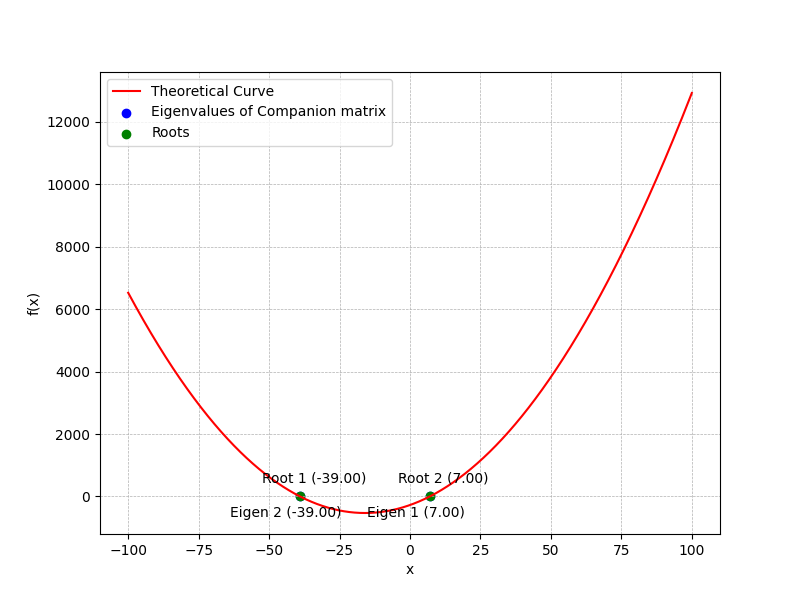
\includegraphics[width=0.8\linewidth]{figs/fig.png}
    \caption{Graph of the quadratic equation.}
\end{figure}
\end{frame}

\end{document}
